\documentclass[10pt,        % Don't change the font size!
               a4paper,     % Don't change the paper size!
               journal,     % Journal paper format
%               draft       % Enable this parameter to get a draft version.
               ]{IEEEtran}
\makeatletter


\def\markboth#1#2{\def\leftmark{\@IEEEcompsoconly{\sffamily}\MakeUppercase{\protect#1}}%
\def\rightmark{\@IEEEcompsoconly{\sffamily}\MakeUppercase{\protect#2}}}
\makeatother

% Use this package for new German hyphenation and to set some 
% captions to German (e.g. Abstract -> Zusammenfassung)
% \usepackage[ngerman]{babel}

% Select input file coding Latin1 or UTF8.
% See "http://en.wikipedia.org/wiki/Latin1" and "http://en.wikipedia.org/wiki/Utf8"
% for more information.
%
%\usepackage[latin1]{inputenc}
\usepackage[utf8]{inputenc}

\usepackage[T1]{fontenc}

\usepackage{booktabs,amsmath}

\usepackage{pgfplots}

\newcommand{\NA}{---}

\definecolor{tumblue}{RGB}{  0, 101, 189}

\usetikzlibrary{chains, positioning, shapes.symbols}
\usepackage{etoolbox}

%
% If IEEEtran.cls has not been installed into the LaTeX system files,
% manually specify the path to it like:
% \documentclass[journal]{../sty/IEEEtran}

% *** GRAPHICS RELATED PACKAGES ***
%
\ifCLASSINFOpdf
  % \usepackage[pdftex]{graphicx}
  % declare the path(s) where your graphic files are
  % \graphicspath{{../pdf/}{../jpeg/}}
  % and their extensions so you won't have to specify these with
  % every instance of \includegraphics
  % \DeclareGraphicsExtensions{.pdf,.jpeg,.png}
\else
  % or other class option (dvipsone, dvipdf, if not using dvips). graphicx
  % will default to the driver specified in the system graphics.cfg if no
  % driver is specified.
  % \usepackage[dvips]{graphicx}
  % declare the path(s) where your graphic files are
  % \graphicspath{{../eps/}}
  % and their extensions so you won't have to specify these with
  % every instance of \includegraphics
  % \DeclareGraphicsExtensions{.eps}
\fi

% *** MATH PACKAGES ***
%
%\usepackage[cmex10]{amsmath}
% A popular package from the American Mathematical Society that provides
% many useful and powerful commands for dealing with mathematics. If using
% it, be sure to load this package with the cmex10 option to ensure that
% only type 1 fonts will utilized at all point sizes. Without this option,
% it is possible that some math symbols, particularly those within
% footnotes, will be rendered in bitmap form which will result in a
% document that can not be IEEE Xplore compliant!
%
% Also, note that the amsmath package sets \interdisplaylinepenalty to 10000
% thus preventing page breaks from occurring within multiline equations. Use:
%\interdisplaylinepenalty=2500
% after loading amsmath to restore such page breaks as IEEEtran.cls normally
% does. amsmath.sty is already installed on most LaTeX systems. The latest
% version and documentation can be obtained at:
% http://www.ctan.org/tex-archive/macros/latex/required/amslatex/math/

% *** SPECIALIZED LIST PACKAGES ***
%
%\usepackage{algorithmic}
% algorithmic.sty was written by Peter Williams and Rogerio Brito.
% This package provides an algorithmic environment fo describing algorithms.
% You can use the algorithmic environment in-text or within a figure
% environment to provide for a floating algorithm. Do NOT use the algorithm
% floating environment provided by algorithm.sty (by the same authors) or
% algorithm2e.sty (by Christophe Fiorio) as IEEE does not use dedicated
% algorithm float types and packages that provide these will not provide
% correct IEEE style captions. The latest version and documentation of
% algorithmic.sty can be obtained at:
% http://www.ctan.org/tex-archive/macros/latex/contrib/algorithms/
% There is also a support site at:
% http://algorithms.berlios.de/index.html
% Also of interest may be the (relatively newer and more customizable)
% algorithmicx.sty package by Szasz Janos:
% http://www.ctan.org/tex-archive/macros/latex/contrib/algorithmicx/

% *** ALIGNMENT PACKAGES ***
%
%\usepackage{array}
% Frank Mittelbach's and David Carlisle's array.sty patches and improves
% the standard LaTeX2e array and tabular environments to provide better
% appearance and additional user controls. As the default LaTeX2e table
% generation code is lacking to the point of almost being broken with
% respect to the quality of the end results, all users are strongly
% advised to use an enhanced (at the very least that provided by array.sty)
% set of table tools. array.sty is already installed on most systems. The
% latest version and documentation can be obtained at:
% http://www.ctan.org/tex-archive/macros/latex/required/tools/


%\usepackage{mdwmath}
%\usepackage{mdwtab}
% Also highly recommended is Mark Wooding's extremely powerful MDW tools,
% especially mdwmath.sty and mdwtab.sty which are used to format equations
% and tables, respectively. The MDWtools set is already installed on most
% LaTeX systems. The lastest version and documentation is available at:
% http://www.ctan.org/tex-archive/macros/latex/contrib/mdwtools/


% IEEEtran contains the IEEEeqnarray family of commands that can be used to
% generate multiline equations as well as matrices, tables, etc., of high
% quality.


%\usepackage{eqparbox}
% Also of notable interest is Scott Pakin's eqparbox package for creating
% (automatically sized) equal width boxes - aka "natural width parboxes".
% Available at:
% http://www.ctan.org/tex-archive/macros/latex/contrib/eqparbox/

% *** SUBFIGURE PACKAGES ***
%\usepackage[tight,footnotesize]{subfigure}
% subfigure.sty was written by Steven Douglas Cochran. This package makes it
% easy to put subfigures in your figures. e.g., "Figure 1a and 1b". For IEEE
% work, it is a good idea to load it with the tight package option to reduce
% the amount of white space around the subfigures. subfigure.sty is already
% installed on most LaTeX systems. The latest version and documentation can
% be obtained at:
% http://www.ctan.org/tex-archive/obsolete/macros/latex/contrib/subfigure/
% subfigure.sty has been superceeded by subfig.sty.



%\usepackage[caption=false]{caption}
%\usepackage[font=footnotesize]{subfig}
% subfig.sty, also written by Steven Douglas Cochran, is the modern
% replacement for subfigure.sty. However, subfig.sty requires and
% automatically loads Axel Sommerfeldt's caption.sty which will override
% IEEEtran.cls handling of captions and this will result in nonIEEE style
% figure/table captions. To prevent this problem, be sure and preload
% caption.sty with its "caption=false" package option. This is will preserve
% IEEEtran.cls handing of captions. Version 1.3 (2005/06/28) and later 
% (recommended due to many improvements over 1.2) of subfig.sty supports
% the caption=false option directly:
%\usepackage[caption=false,font=footnotesize]{subfig}
%
% The latest version and documentation can be obtained at:
% http://www.ctan.org/tex-archive/macros/latex/contrib/subfig/
% The latest version and documentation of caption.sty can be obtained at:
% http://www.ctan.org/tex-archive/macros/latex/contrib/caption/

% *** FLOAT PACKAGES ***
%
%\usepackage{fixltx2e}
% fixltx2e, the successor to the earlier fix2col.sty, was written by
% Frank Mittelbach and David Carlisle. This package corrects a few problems
% in the LaTeX2e kernel, the most notable of which is that in current
% LaTeX2e releases, the ordering of single and double column floats is not
% guaranteed to be preserved. Thus, an unpatched LaTeX2e can allow a
% single column figure to be placed prior to an earlier double column
% figure. The latest version and documentation can be found at:
% http://www.ctan.org/tex-archive/macros/latex/base/



%\usepackage{stfloats}
% stfloats.sty was written by Sigitas Tolusis. This package gives LaTeX2e
% the ability to do double column floats at the bottom of the page as well
% as the top. (e.g., "\begin{figure*}[!b]" is not normally possible in
% LaTeX2e). It also provides a command:
%\fnbelowfloat
% to enable the placement of footnotes below bottom floats (the standard
% LaTeX2e kernel puts them above bottom floats). This is an invasive package
% which rewrites many portions of the LaTeX2e float routines. It may not work
% with other packages that modify the LaTeX2e float routines. The latest
% version and documentation can be obtained at:
% http://www.ctan.org/tex-archive/macros/latex/contrib/sttools/
% Documentation is contained in the stfloats.sty comments as well as in the
% presfull.pdf file. Do not use the stfloats baselinefloat ability as IEEE
% does not allow \baselineskip to stretch. Authors submitting work to the
% IEEE should note that IEEE rarely uses double column equations and
% that authors should try to avoid such use. Do not be tempted to use the
% cuted.sty or midfloat.sty packages (also by Sigitas Tolusis) as IEEE does
% not format its papers in such ways.


%\ifCLASSOPTIONcaptionsoff
%  \usepackage[nomarkers]{endfloat}
% \let\MYoriglatexcaption\caption
% \renewcommand{\caption}[2][\relax]{\MYoriglatexcaption[#2]{#2}}
%\fi
% endfloat.sty was written by James Darrell McCauley and Jeff Goldberg.
% This package may be useful when used in conjunction with IEEEtran.cls'
% captionsoff option. Some IEEE journals/societies require that submissions
% have lists of figures/tables at the end of the paper and that
% figures/tables without any captions are placed on a page by themselves at
% the end of the document. If needed, the draftcls IEEEtran class option or
% \CLASSINPUTbaselinestretch interface can be used to increase the line
% spacing as well. Be sure and use the nomarkers option of endfloat to
% prevent endfloat from "marking" where the figures would have been placed
% in the text. The two hack lines of code above are a slight modification of
% that suggested by in the endfloat docs (section 8.3.1) to ensure that
% the full captions always appear in the list of figures/tables - even if
% the user used the short optional argument of \caption[]{}.
% IEEE papers do not typically make use of \caption[]'s optional argument,
% so this should not be an issue. A similar trick can be used to disable
% captions of packages such as subfig.sty that lack options to turn off
% the subcaptions:
% For subfig.sty:
% \let\MYorigsubfloat\subfloat
% \renewcommand{\subfloat}[2][\relax]{\MYorigsubfloat[]{#2}}
% For subfigure.sty:
% \let\MYorigsubfigure\subfigure
% \renewcommand{\subfigure}[2][\relax]{\MYorigsubfigure[]{#2}}
% However, the above trick will not work if both optional arguments of
% the \subfloat/subfig command are used. Furthermore, there needs to be a
% description of each subfigure *somewhere* and endfloat does not add
% subfigure captions to its list of figures. Thus, the best approach is to
% avoid the use of subfigure captions (many IEEE journals avoid them anyway)
% and instead reference/explain all the subfigures within the main caption.
% The latest version of endfloat.sty and its documentation can obtained at:
% http://www.ctan.org/tex-archive/macros/latex/contrib/endfloat/
%
% The IEEEtran \ifCLASSOPTIONcaptionsoff conditional can also be used
% later in the document, say, to conditionally put the References on a 
% page by themselves.

% correct bad hyphenation here
\hyphenation{op-tical net-works semi-conduc-tor}


\begin{document}
\title{Neural Architecture Search for Automated Machine Learning Deployment on Extreme Edge Devices}
%
% author names and IEEE memberships
% note positions of commas and nonbreaking spaces ( ~ ) LaTeX will not break
% a structure at a ~ so this keeps an author's name from being broken across
% two lines.
% use \thanks{} to gain access to the first footnote area
% a separate \thanks must be used for each paragraph as LaTeX2e's \thanks
% was not built to handle multiple paragraphs
%

\author{Philipp van Kempen, Technische Universit\"at M\"unchen, Munich, Germany} % <-this % stops a space

%\thanks{M. Shell is with the Department
%of Electrical and Computer Engineering, Georgia Institute of Technology, Atlanta,
%GA, 30332 USA e-mail: (see http://www.michaelshell.org/contact.html).}% <-this % stops a space
%\thanks{J. Doe and J. Doe are with Anonymous University.}% <-this % stops a space
%\thanks{Manuscript received April 19, 2005; revised January 11, 2007.}}

% note the % following the last \IEEEmembership and also \thanks - 
% these prevent an unwanted space from occurring between the last author name
% and the end of the author line. i.e., if you had this:
% 
% \author{....lastname \thanks{...} \thanks{...} }
%                     ^------------^------------^----Do not want these spaces!
%
% a space would be appended to the last name and could cause every name on that
% line to be shifted left slightly. This is one of those "LaTeX things". For
% instance, "\textbf{A} \textbf{B}" will typeset as "A B" not "AB". To get
% "AB" then you have to do: "\textbf{A}\textbf{B}"
% \thanks is no different in this regard, so shield the last } of each \thanks
% that ends a line with a % and do not let a space in before the next \thanks.
% Spaces after \IEEEmembership other than the last one are OK (and needed) as
% you are supposed to have spaces between the names. For what it is worth,
% this is a minor point as most people would not even notice if the said evil
% space somehow managed to creep in.

% The paper headers
\markboth{Advanced Seminar - Real-Time Computer Systems, Winter Term 2020}%
{Philipp van Kempen: Network Architecture Search for Automated Machine Learning Deployment on Extreme Edge Devices}

%\markboth{Journal of \LaTeX\ Class Files,~Vol.~6, No.~1, January~2007}%
%{Shell \MakeLowercase{\textit{et al.}}: Bare Demo of IEEEtran.cls for Journals}
% The only time the second header will appear is for the odd numbered pages
% after the title page when using the twoside option.
% 
% *** Note that you probably will NOT want to include the author's ***
% *** name in the headers of peer review papers.                   ***
% You can use \ifCLASSOPTIONpeerreview for conditional compilation here if
% you desire.

% If you want to put a publisher's ID mark on the page you can do it like
% this:
%\IEEEpubid{0000--0000/00\$00.00~\copyright~2007 IEEE}
% Remember, if you use this you must call \IEEEpubidadjcol in the second
% column for its text to clear the IEEEpubid mark.

% use for special paper notices
%\IEEEspecialpapernotice{(Invited Paper)}

% make the title area
\maketitle


\begin{abstract}
%\boldmath
%Put the abstract here. The abstract should be 200-300 words long and must
%answer the following questions:
%\begin{itemize}
%   \item Why is this topic important and interesting?
%   \item What is the topic?
%\end{itemize}
%It's a good writing style to answer the "why" question first by putting the
%topic in a broader context. 
Machine Learning and Artificial Intelligence are omnipresent topics nowadays. Especially since small personal devices, such as smartphones, are capable of running this computation intensive tasks on their own, they can improve our lives in many different ways, e.g. computer vision or speech detection.
Deploying neural network models on tiny and therefore performance-, memory- and power-constrained devices, such as microcontrollers, is currently an important research topic. For mobile and other embedded target devices Neural Architecture Search (NAS) is a new method to find appropriate network models without requiring manual error-prone adjustments by engineers, which allows to automate the workflow from the definition of a real work problem to a deployable solution \cite{nassurvey}. While there are a lot of comprehensive surveys on NAS methods in general \cite{nassurvey,wsnas2020}, none of them considers the application of those ideas on edge devices like microcontrollers (MCUs). This work provides an overview of the recent developments and compares different approaches, which appeared over the last few years, against one another and with well-known reference applications intended for the usage on mobile phones. In the end some opportunities for future work on this topic are discussed.

\end{abstract}
% IEEEtran.cls defaults to using nonbold math in the Abstract.
% This preserves the distinction between vectors and scalars. However,
% if the journal you are submitting to favors bold math in the abstract,
% then you can use LaTeX's standard command \boldmath at the very start
% of the abstract to achieve this. Many IEEE journals frown on math
% in the abstract anyway.

% Note that keywords are not normally used for peerreview papers.
%\begin{IEEEkeywords}
%IEEEtran, journal, \LaTeX, paper, template.
%\end{IEEEkeywords}



% For peer review papers, you can put extra information on the cover
% page as needed:
% \ifCLASSOPTIONpeerreview
% \begin{center} \bfseries EDICS Category: 3-BBND \end{center}
% \fi
%
% For peerreview papers, this IEEEtran command inserts a page break and
% creates the second title. It will be ignored for other modes.
% \IEEEpeerreviewmaketitle
\setlength{\tabcolsep}{2pt}

\section{Introduction}\label{sec:intro}
%In general a scientific paper starts with an introduction to the topic.

The training of large machine learning models is typically done on specific high-performance computers, but may still require a lot of time. This makes is hard to tune hyper-parameters or the model architecture in an intensive way. Therefore a way to reduce the design time human interaction and know-how is needed. This is not the case for smaller models targeting embedded systems as their architecture is often much simpler resulting in training times of just a few minutes for mid-size applications. Finding the best suitable model architecture to run on  edge devices, which are known to have several resource constraints like computational power and memory size with typical values in the range of several KB to very few MB, is currently a highly relevant topic being explored by many researchers worldwide. After a brief introduction of some core concepts of Machine Learning like NAS, AutoML and available Frameworks, a survey on papers on the aforementioned subject follows in section \ref{sec:sota}. The benchmark results for these approaches are compared as far as possible in section \ref{sec:comp} before the core results and ideas for further work on the topics are summarized in section \ref{sec:con}.

\subsection{Neural Architecture Search and AutoML}
Short training times enable the application of optimization techniques to either improve the accuracy or the size of the resulting models in a meaningful way. Especially Neural Architecture Search methods benefit of such targets as they allow many design iterations and therefore more promising results in shorter time. AutoML workflows, which combine NAS with further automated process steps as shown in figure \ref{fig:automl}, are already being used in research groups and will become more relevant for the future AI industry \cite{automl2019}. While Data Preparation and Feature Engineering are prerequisite steps to apply NAS, automated machine learning may make full use of potential of Neural Architecture Search during the generation and estimation of models. Search space exploration and optimization methods like heuristics or evolutionary algorithms may be used to gain architectures fulfilling the given constraints. There are many methods which can be used for model compression in the final estimation step, where weight-sharing is one of the most relevant ones. In the method of weight-sharing a larger super-network is typically trained to provide a higher number of possible sub-networks for evaluation. This reduces the search cost as the parameters of overlapping sub-networks are only computed once \cite{Chu2019}. Other approaches to reduce the model complexity are the quantization of floating point model state values and parameters to smaller fixed-point data types or pruning which removes a certain amount of parameters determined by a given pruning method \cite{Molchanov2019}.

\begin{figure*}
    \centering
    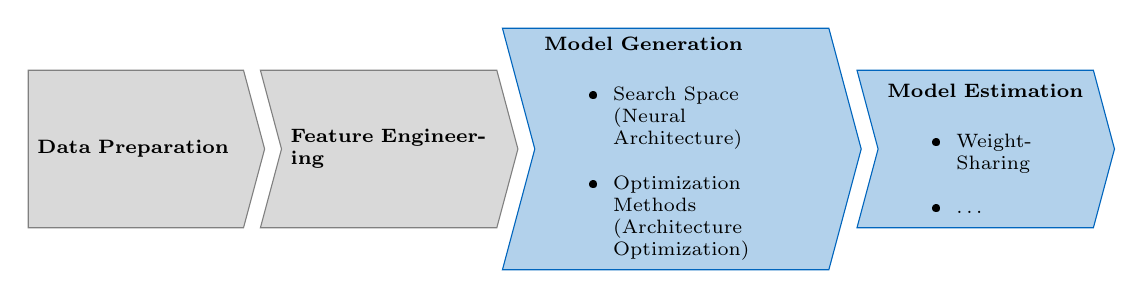
\begin{tikzpicture}[
node distance = 2mm,
  start chain = going right,
 start/.style = {signal, draw=#1, fill=#1!30,
                 text width=25mm, minimum height=20mm, font=\scriptsize,
                 signal pointer angle=150, on chain},
  cont/.style = {start=#1, signal from=west}
                 ]

\node[start=gray] {\bfseries
                     Data Preparation\\
                        };
\node[cont=gray] {\bfseries
                     Feature Engineering\\
                        };
\node[cont=tumblue,text width=35mm] {\bfseries
                     Model Generation\\[1ex]
                     \normalfont
                        \begin{itemize}
                    \item Search Space\\(Neural Architecture)
                    \item Optimization Methods\\(Architecture Optimization)
                        \end{itemize} };
                     
\node[cont=tumblue] {\bfseries
                     Model Estimation\\[1ex]
                     \normalfont
                        \begin{itemize}
                    \item Weight-Sharing
                    \item \ldots
                        \end{itemize} };
\end{tikzpicture}
    \caption{Typical AutoML Flow \cite{automl2019} (Highlighted Steps are relevant for NAS)}
    \label{fig:automl}
\end{figure*}

\subsection{Frameworks}

To design machine learning models and deploy them on a target device some framework or library is typically used. As later shown in this paper, this choice can have a large impact on the performance and size of the resulting design. Especially the ``engine'' used for running the inference on a microcontroller device may be a bottleneck or provide some room for improvements. While Tensorflow Lite (TFLite) mostly targets mobile devices, there is a relatively novel but popular library called Tensorflow Lite Micro (TFLM) with kernels, e.g. methods to execute operations of the model graph, specialized to resource constrained architectures \cite{tflm2020}. The term TinyML is often used in the context of TFLM but may also refer to machine learning models running on edge devices in general. Custom kernels often referred as CMSIS-NN exist for some targets with hardware accelerators for typical Digital Signal Processing (DSP) instructions using neural network calculations like Multiply and Accumulate \cite{cmsisnn2018}. The data in table \ref{tbl:frameworks} also presents the relevance of both frameworks compared to less widely used MicroTVM and Pytorch, which are not going to be discussed here. Each completely custom framework proposed in a paper has to be compared to the aforementioned state of the art approaches.

\begin{table}[t!]
    \centering
    \footnotesize
        \caption{Frameworks used in the discussed papers ($\circ$: comparisons only)}
    \label{tbl:frameworks}
    \begin{tabular}{cccccc}
  \toprule
  \textbf{Frameworks} & TFLite (Micro) &  CMSIS-NN & MicroTVM & Pytorch & Custom  \\
  \midrule
  \textit{MCUNet}\cite{mcunet2020} & $\circ$ & $\circ$ & $\circ$ & & $\bullet$\\
  \textit{$\mu$NAS}\cite{unas2020} & $\bullet$ & $\bullet$ & & & \\
  \textit{SpArSe}\cite{sparse2019} & N/A & N/A & N/A & N/A & N/A\\
  \textit{MicroNets}\cite{micronets2020} & $\bullet$ & $\bullet$ & & & \\
  \textit{Once-for-All}\cite{once4all2019} & & & & $\bullet$ &\\
  \bottomrule
\end{tabular}
\end{table}


\section{State of the Art}\label{sec:sota}
Although the following brief overview on research papers focuses on the proposed NAS methods instead of the inference engine or model types, the framework used for the design and deployment sometimes also need consideration due to specific model-optimizations, which may only have certain effects when applied together with the suitable counterparts.

Beside frameworks there exist many research results on NAS performance for popular reference models like ImageNet \cite{imagenet2009} and CIFAR-10 \cite{cifar10}. Unfortunately they are initially targeted to devices offering more computing power. Due to their large size or operation count (computational demand) not all of them are suitable for comparing NAS results on microcontrollers. To demonstrate the possibilities of machine learning on edge devices some popular application spaces like Image Recognition (ImageNet), Visual Wake Words and Speech Commands (Keyword Spotting, KWS), can be used. There also exist many datasets for the classification of handwritten characters or digits (MNIST). Applications like Anomaly Detection or DSP Classification have higher relevance for the real world but often lack of representative datasets, hence why they are only used in some of the research papers.

%COLLECTION OF CITES:  \cite{dory2020}   \cite{opreordering2019}

% needed in second column of first page if using \IEEEpubid
%\IEEEpubidadjcol

%\subsubsection{Subsubsection Heading Here}
%Subsubsection text here.

\subsection{MCUNet}

The MCUNet system-model co-design framework consists of two main components. The first one is a Neural Architecture Search algorithm suitable for MCUs and a lightweight inference engine based on code generation. The latter is called TinyEngine and profits of memory scheduling, which takes the overall network topology into account instead of only considering individual layers for optimization. This leads to smaller models in terms of memory requirements and operation count and therefore to an increase of the size of the NAS search space. The two-stage algorithm of the so called TinyNAS component optimizes the aforementioned search space according to given resource constraints before specializing its properties to handle various constraints at once \cite{mcunet2020}. Inference results in comparison with the state of the art Tensorflow Lite Micro library and CMSIS-NN \cite{cmsisnn2018} are presented in section \ref{sec:comp}.

TinyNAS at first searches for the best search space configuration $S*$ in the set of possible configuration $S$ which is a non-trivial task. By using the cummulative-distribution-function (CDF) of FLOPS instead of the CDF of model accuracy the high cost of training each network can be avoided. One-shot architecture search making use of weight sharing in combination with evolutionary search determines the resulting model suitable for the given set of constraints.

By performing in-place depth-wise convolutions using a single temporal buffer, TinyEngine can reduce the peak memory for $N$ channels from $2N$ to $N+1$. Additionally methods such as adaptive scheduling or loop unrolling are applied on parts of the model architecture during code generation to reduce the number of required operations for running a neural network model. \cite{mcunet2020}


\subsection{$\mu$NAS}

Similar to TinyNAS, $\mu$NAS generates mid-tier MCU-level networks with sizes from 0.5 KB to 64 KB, which are primarily intended for image classification tasks. Multi-objective optimization takes RAM-size, persistent storage and processor speed into account \cite{unas2020}. The experiment results in the recently published paper already featuring comparisons with for example the MCUNet framework.

Different to traditional approaches for GPU- or mobile-level NAS design, $\mu$NAS was designed following two special design requirements: A highly granular search space and the accurate computation of used resources. The resulting four-step search procedure is based on the concepts of aging evolution and pruning and is briefly shown in figure \ref{fig:unas}.

\begin{figure}
    \centering
    \includegraphics[scale=0.75]{paper/figures/unas.pdf}
    \caption{General search procedure for $\mu$NAS \cite{unas2020}}
    \label{fig:unas}
\end{figure}

\subsection{SpArSe}

To demonstrate the possibility of designing Convolutional Neural Networks (CNNs) which generalize well via AutoML, while still being small enough to fit onto memory-constrained MCUs, \cite{sparse2019} proposes an architecture search method combining neural architecture search with pruning. The resulting applications for the IoT field definitely display a success of the aforementioned challenge. 

Using a balanced multi-objective optimization problem operating on the problem space $\Omega=\{\alpha,\theta,\omega,\Theta\}$ composed of the network connectivity graph $\alpha$, network weights $\omega$, operations $\theta$ and training hyper-parameters $\Theta$ small but performant CNNs can be generated. The three objective functions

\begin{itemize}
    \item $f_1(\Omega)=1-\textsc{ValidationAccuracy}(\Omega)$
    \item $f_2(\Omega)=\textsc{ModelSize}(\Omega)$
    \item $f_3(\Omega) =\max_{l \in 1,\ldots,L} \textsc{WorkingMemory}_l(\Omega)$
\end{itemize}

 are used to design the SpArSe architectures with $L$ being the number of network layers. After a model size compression via pruning the best suitable sub-spaces are determined using Bayesian optimization. Instead of weight-sharing, Network morphism is applied in combination with random scalarizations  \cite{sparse2019} to evaluate each configuration $\Omega^n$ at low computational costs.

\subsection{MicroNets}

To employ a new differentiable NAS (DNAS) realization for edge devices with tight memory and performance constraints in \cite{micronets2020} the properties of NAS search spaces for MCU model design were studied first. The most important result of this step is the correlation between the model latency and the model operation count under a uniform prior over models in the search space. Therefore the op count is used as viable proxy to latency when searching for the optimal network architecture. Designed models can target three different size-classes (S/M/L). Another aspect of NAS is the underlying latency/energy model which is also mentioned in \cite{micronets2020}. TinyML performance for industry standard benchmarks is shortly mentioned in \ref{sec:comp}.

After deriving the correlation between the layer operation count and the layer latency and the energy model the paper proposes MircoNet Models following a DNAS approach. Instead of using model constraints to restrict the feasible space, regularization terms are incorporated in the DNAS objective function. Compression techniques such as `Sub-Byte' quantization follow. \cite{micronets2020}

\subsection{Once-for-All (OFA)}

While the generation and inference of models especially designed for microcontrollers was the main objective in the previously mentioned works, the Once-for-All approach \cite{once4all2019} is built to design optimal networks suitable for a wide range of devices. Usually this is a costly goal as training one model for each architectural settings is required. By decoupling the training and search, it is possible to get a sub network which can be then optimized in multiple dimensions like depth, width and kernel size. As a novel progressive shrinking algorithm, a generalized pruning algorithm is proposed and state-of-the-art performance especially for the mobile setting presented.

The following special CNN techniques are applied in the OFA search space generation process to create a single large Once-for-All network.

\begin{itemize}
    \item \textbf{Elastic depth:} arbitrary numbers of layers per unit
    \item \textbf{Elastic width:} arbitrary numbers of channels per layer
    \item \textbf{Elastic kernel size:} arbitrary kernel sizes
    \item \textbf{Elastic resolution:} arbitrary input image sizes
\end{itemize}

Smaller sub-networks can make use of this trained OFA network by exploiting weight sharing and progressive shrinking. In the deployment stage no additional expensive training time is required due to the decoupling. \cite{once4all2019}



%\section{Please Note}
%Regular research papers need at least two additional %sections here. One section
%for contributions and methods and one section for the %results. For seminar
%papers these sections can be omitted. 

\section{Comparison}\label{sec:comp}

There are a lot of metrics to evaluate how the proposed NAS methods improve or degrade the performance of the resulting models. Often the model accuracy after deployment and the size of the generated program are primarily considered because of the given tight memory constrains in terms of program memory and SRAM usage on edge devices. If inference latency or frequency is relevant, the execution time, count of instructions or number of Multiply or Accumulate operations will be taken into account. This is a more accurate approach than counting Floating Point Operations (FLOPS) on embedded systems. It may also be helpful to evaluate metrics like training time, search cost or even the resulting energy consumption as done in paper \cite{once4all2019}.

ProxylessNAS is proposed in \cite{proxyless2018} and mainly focuses on mobile target devices. It is not included in the previous section but shortly explained here as three of the MCU-class NAS approaches mention it as a reference design. In \cite{ai2edge2020} a survey on deep learning techniques, which are critical for edge intelligence implementation, statements on the performance of MCUNet, Sparse and OFA can be found. Unfortunately the table is missing important information such as the search cost.

By using the MCUNet framework instead of Tensorflow Lite Micro and CMSIS-NN the required amount of MCU-memory drops by the large factor of $3.4$ while the inference time is $1.7$- to $3.3$-times shorter  \cite{mcunet2020}. This achievement is likely due to the interpreter based inference engine used in the TFLite Micro Library which introduces a large memory overhead compared to TinyEngine's code-generation approach. In addition the layer-level optimization strategies which are used in the MicroTVM framework as well are sub-optimal, which lead to further advantages for MCUNet. \cite{mcunet2020}.

Model accuracy was first evaluated by comparing top1 ImageNet results which achieved >70\% on common microcontrollers. Meanwhile the required SRAM memory and flash compared to quantized MobileNetV2 and ResNet-18 is $3.5$ or $5.7$ times smaller and especially for visual and audio wake words, which are popular reference implementations, the MCUNet framework is faster and also smaller than MobileNetV2 and ProxylessNAS-based solutions \cite{mcunet2020}.

Experiments with $\mu$NAS have been conducted on image classification data sets. Either the top-1 classification accuracy can be increased by up to $4.8\%$, the memory footprint can be lowered by $4$–$13$ times or alternatively a reduction of the number of multiply-accumulate operations by $\approx$ $900\times$ is possible according to \cite{unas2020}. Further interesting numbers can be found in a table of pareto-optimal architectures as it can be seen that $\mu$NAS outperforms SpArSe in multiple character classification

SpArSe achieves to provide a more accurate and up to $4.35\times$ smaller models compared to previous approaches on IoT data sets. Unfortunately no comparisons with either of the other papers are available, hence why performance on standard datasets and the Bonsai-Net paper \cite{Geada2020} are the only references in this case. Character classification with SpArSe turned out to to have similar higher accuracy or drastically lower memory requirements and network sizes. 

MicroNet models have been deployed on MCUs to compete with Tensorflow Lite Micro in experiments. Visual wake words, audio keyword spotting and anomaly detection have been compared with MobileNetV2, ProxylessNAS, Tensorflow Lite Micro and MSNET \cite{micronets2020}.\\
The paper also states the pareto optimality of MicroNet models against MCUNet for KWS tasks.

Using the Once-for-All tools over $1000$ sub-networks suitable to run on several constrained target hardware platforms could be obtained. Regardless of the actual latency constrains it was possible to maintain the level of accuracy after the initial training. Actual numbers are provided for ImageNet top-1 accuracy under the mobile setting with sub-$600$ million Multiply-Accumulate operations for running the network while achieving an accuracy of $80\%$ \cite{once4all2019}.

Even on edge devices the results are promising as either an increase of ImageNet top1 accuracy by $4.0\%$ or a $1.5-2.6$ times lower latency compared with MobileNetV3 and EfficientNet at constant accuracy level is possible.
It is emphasized that the amount of GPU hours for training also drops by many orders of magnitude resulting in less CO2 emission \cite{once4all2019}.

% An example of a floating figure using the graphicx package.
% Note that \label must occur AFTER (or within) \caption.
% For figures, \caption should occur after the \includegraphics.
% Note that IEEEtran v1.7 and later has special internal code that
% is designed to preserve the operation of \label within \caption
% even when the captionsoff option is in effect. However, because
% of issues like this, it may be the safest practice to put all your
% \label just after \caption rather than within \caption{}.
%
% Reminder: the "draftcls" or "draftclsnofoot", not "draft", class
% option should be used if it is desired that the figures are to be
% displayed while in draft mode.
%
%\begin{figure}[!t]
%\centering
%\includegraphics[width=2.5in]{myfigure}
% where an .eps filename suffix will be assumed under latex, 
% and a .pdf suffix will be assumed for pdflatex; or what has been declared
% via \DeclareGraphicsExtensions.
%\caption{Simulation Results}
%\label{fig_sim}
%\end{figure}

% Note that IEEE typically puts floats only at the top, even when this
% results in a large percentage of a column being occupied by floats.


% An example of a double column floating figure using two subfigures.
% (The subfig.sty package must be loaded for this to work.)
% The subfigure \label commands are set within each subfloat command, the
% \label for the overall figure must come after \caption.
% \hfil must be used as a separator to get equal spacing.
% The subfigure.sty package works much the same way, except \subfigure is
% used instead of \subfloat.
%
%\begin{figure*}[!t]
%\centerline{\subfloat[Case I]\includegraphics[width=2.5in]{subfigcase1}%
%\label{fig_first_case}}
%\hfil
%\subfloat[Case II]{\includegraphics[width=2.5in]{subfigcase2}%
%\label{fig_second_case}}}
%\caption{Simulation results}
%\label{fig_sim}
%\end{figure*}
%
% Note that often IEEE papers with subfigures do not employ subfigure
% captions (using the optional argument to \subfloat), but instead will
% reference/describe all of them (a), (b), etc., within the main caption.


% An example of a floating table. Note that, for IEEE style tables, the 
% \caption command should come BEFORE the table. Table text will default to
% \footnotesize as IEEE normally uses this smaller font for tables.
% The \label must come after \caption as always.
%
%\begin{table}[!t]
%% increase table row spacing, adjust to taste
%\renewcommand{\arraystretch}{1.3}
% if using array.sty, it might be a good idea to tweak the value of
% \extrarowheight as needed to properly center the text within the cells
%\caption{An Example of a Table}
%\label{table_example}
%\centering
%% Some packages, such as MDW tools, offer better commands for making tables
%% than the plain LaTeX2e tabular which is used here.
%\begin{tabular}{|c||c|}
%\hline
%One & Two\\
%\hline
%Three & Four\\
%\hline
%\end{tabular}
%\end{table}


% Note that IEEE does not put floats in the very first column - or typically
% anywhere on the first page for that matter. Also, in-text middle ("here")
% positioning is not used. Most IEEE journals use top floats exclusively.
% Note that, LaTeX2e, unlike IEEE journals, places footnotes above bottom
% floats. This can be corrected via the \fnbelowfloat command of the
% stfloats package.


%\section{Fazit}
\section{Conclusion}\label{sec:con}
To summarize the results of the recent work on Neural Architecture Search for edge devices, it is easy to see that it is an highly relevant research topic which offers a lot of innovation for the future AI industry. 

The biggest improvements compared to reference models can been acquired if the NAS algorithm is co-designed with the corresponding inference engine. The reason for this is that a larger search space provides more opportunities to find optimal designs, due to faster model invocation.

All approaches are published under an open-source license which should allow other researchers to built up on these work to obtain even better results. For example Tensorflow Lite Micro, which is the most relevant microcontrollers inference framework, could profit a lot if NAS would be integrated in the design workflow. Beside the reusability improvement this could also make it easier to gather data for comparisons with other approaches.

There are a lot of other relevant research results on lightweight machine learning unrelated to NAS which use optimization techniques such as mixed low bitwidth quantization \cite{memorydrivenquant2019}. Implementing CNNs on MCUs with standard convolutions instead of depth-wise convolutions by trading accuracy with computational cost also offers appealing results as proposed in \cite{mixedquant2020}. Another model compression method is proposed in \cite{opreordering2019} and uses a reordering of the model moderation to reduce its memory footprint.

%Proposals of me: \cite{wsnas2020} (meniones DARTS, use later?), \cite{mixedquant2020} (image classification, hand crafted: mobilenetv1, mobilenetv2, shufflenet, nas methods use RL or backpropagation i.e. DNAS, complementary (ergänzend) to NAS), \cite{iotnet2019} (standard conv instead of depth-wise conv, trade accuracy with computational cost), \cite{memorydrivenquant2019} (mixed low bitwidth qaunt, 2/4/8 bit, on mcu, using mobilenetv1)

% if have a single appendix:
%\appendix[Proof of the Zonklar Equations]
% or
%\appendix  % for no appendix heading
% do not use \section anymore after \appendix, only \section*
% is possibly needed

% use appendices with more than one appendix
% then use \section to start each appendix
% you must declare a \section before using any
% \subsection or using \label (\appendices by itself
% starts a section numbered zero.)
%


% \appendices
% \section{Proof of the First Zonklar Equation}
% Appendix one text goes here.

% you can choose not to have a title for an appendix
% if you want by leaving the argument blank
% \section{}
% Appendix two text goes here.


% use section* for acknowledgement
%\section*{Acknowledgment}


%The authors would like to thank...


% Can use something like this to put references on a page
% by themselves when using endfloat and the captionsoff option.
\ifCLASSOPTIONcaptionsoff
  \newpage
\fi



% trigger a \newpage just before the given reference
% number - used to balance the columns on the last page
% adjust value as needed - may need to be readjusted if
% the document is modified later
%\IEEEtriggeratref{8}
% The "triggered" command can be changed if desired:
%\IEEEtriggercmd{\enlargethispage{-5in}}

% references section

% can use a bibliography generated by BibTeX as a .bbl file
% BibTeX documentation can be easily obtained at:
% http://www.ctan.org/tex-archive/biblio/bibtex/contrib/doc/
% The IEEEtran BibTeX style support page is at:
% http://www.michaelshell.org/tex/ieeetran/bibtex/
%\bibliographystyle{IEEEtran}
% argument is your BibTeX string definitions and bibliography database(s)
%\bibliography{IEEEabrv,../bib/paper}
%
% <OR> manually copy in the resultant .bbl file
% set second argument of \begin to the number of references
% (used to reserve space for the reference number labels box)
%\begin{thebibliography}{1}
%
%\bibitem{IEEEhowto:kopka}
%H.~Kopka and P.~W. Daly, \emph{A Guide to \LaTeX}, 3rd~ed.\hskip 1em %plus
%  0.5em minus 0.4em\relax Harlow, England: Addison-Wesley, 1999.
%
%\end{thebibliography}
\bibliographystyle{IEEEtran}
\bibliography{IEEEabrv,references}

% biography section
% 
% If you have an EPS/PDF photo (graphicx package needed) extra braces are
% needed around the contents of the optional argument to biography to prevent
% the LaTeX parser from getting confused when it sees the complicated
% \includegraphics command within an optional argument. (You could create
% your own custom macro containing the \includegraphics command to make things
% simpler here.)
%\begin{biography}[{\includegraphics[width=1in,height=1.25in,clip,keepaspectratio]{mshell}}]{Michael Shell}
% or if you just want to reserve a space for a photo:

%\begin{IEEEbiography}{Michael Shell}
%Biography text here.
%\end{IEEEbiography}

% if you will not have a photo at all:
%\begin{IEEEbiographynophoto}{John Doe}
%Biography text here.
%\end{IEEEbiographynophoto}

% insert where needed to balance the two columns on the last page with
% biographies
%\newpage

%\begin{IEEEbiographynophoto}{Jane Doe}
%Biography text here.
%\end{IEEEbiographynophoto}

% You can push biographies down or up by placing
% a \vfill before or after them. The appropriate
% use of \vfill depends on what kind of text is
% on the last page and whether or not the columns
% are being equalized.

%\vfill

% Can be used to pull up biographies so that the bottom of the last one
% is flush with the other column.
%\enlargethispage{-5in}

\end{document}


